\documentclass[12pt, twoside]{report}
\usepackage{blindtext}
\usepackage[utf8]{inputenc}
\usepackage{graphicx}
\graphicspath{{recursos/}}
\usepackage{float}
\usepackage[letterpaper,top=20mm,bottom=20mm,left=24mm,right=24mm,bindingoffset=0mm]{geometry}
\usepackage[section]{placeins}
\usepackage{booktabs}
\usepackage[spanish,es-nodecimaldot,es-tabla]{babel}
\usepackage{tikz} 
\usepackage{tocloft}
\usepackage{setspace}
\usepackage[nottoc]{tocbibind}
\usepackage{caption}
\usepackage{subcaption}
\usepackage{threeparttable}
\usepackage{acro}
\usepackage{dsfont}
\usepackage{lastpage}
\usepackage{makecell}
\usepackage{tasks}
\usepackage{fancyhdr}
\pagestyle{fancy}
\fancyhead{}
\fancyhead[RO,LE]{Control basado en navegación inercial para un brazo robótico articulado}
\fancyfoot{}
\fancyfoot[LE,RO]{\thepage}
\fancyfoot[CO,CE]{Nicolas Castañeda David Emmanuel}
\renewcommand{\headrulewidth}{0.4pt}
\renewcommand{\footrulewidth}{0.4pt} 
\usepackage{amsmath}
\usepackage{amssymb,amsthm,listings}
\usepackage{braket,lipsum,titlesec}
\usepackage{cleveref,setspace}
\makeatletter
\renewcommand*\env@matrix[1][*\c@MaxMatrixCols c]{%
  \hskip -\arraycolsep
  \let\@ifnextchar\new@ifnextchar
  \array{#1}}
\makeatother
\usepackage{dcolumn}
\newcolumntype{d}{D{-}{-}{0}}
\usepackage{xcolor}
\definecolor{Sepia}{RGB}{111,78,55}
\definecolor{Black}{RGB}{0,0,0}
\usepackage{makeidx}
\makeindex
\usepackage{booktabs}
\usepackage{array}
\usepackage{cite}
\usepackage{gensymb}
\usepackage{textcomp}
\setlength{\headheight}{14.5pt}

\begin{document}

\newgeometry{top=10mm,bottom=5mm,left=0mm,right=0mm}

\thispagestyle{empty}
\begin{minipage}[c][0.17\textheight][c]{0.22\textwidth}
	\begin{center}
		\includegraphics[scale=0.25]{logo-ipn-guinda.png}
	\end{center}
\end{minipage}
\begin{minipage}[c][0.195\textheight][c]{0.71\textwidth}
	\begin{center}
		\vspace{0.3cm}
		\textbf{\Large INSTITUTO POLIT\'ECNICO NACIONAL}
		\vspace{0.4cm}
		\color{Black}\hrule height1pt
		\vspace{0.2cm}
		{\color{Black}\hrule height1pt}
		\vspace{0.4cm}
		\color{Black}\textbf{\textsc{ESCUELA SUPERIOR DE INGENIER\'IA MEC\'ANICA Y EL\'ECTRICA}}
		\textbf{\textsc{Unidad Culhuac\'an\\}}
		\textsc{Ingenier\'ia en Computaci\'on}\\[0.5cm] %
	\end{center}
\end{minipage}

\begin{minipage}[c][0.81\textheight][t]{0.22\textwidth}
	\begin{center}
		\color{Black}\vrule width1pt height16cm 
		\vspace{5mm}
		\hskip2pt
		\color{Black}\vrule width1pt height16cm
		\hskip2mm
		\color{Black}\vrule width1pt height16cm \\
		\includegraphics[scale=0.14]{recursos/esime.png}
	\end{center}
\end{minipage}
\begin{minipage}[c][0.70\textheight][t]{0.7\textwidth}
	\begin{center}
		\vspace{1.5cm}
		
		{\Huge\scshape Control basado en navegaci\'on inercial para un brazo rob\'otico articulado}
		
		\vspace{3.5cm}            
		
		\textsc{\LARGE T   E   S   I   N   A}\\[0.5cm]
		\textsc{\large que para obtener el t\'itulo de}\\[0.5cm]
		\textsc{\large Ingeniero en Computaci\'on}\\[0.5cm]
		\textsc{\large presenta}\\[0.5cm]
		\textsc{\large Nicolas Castañeda David Emmanuel}\\[2cm]          
		
		\vspace{1cm}
		
	\end{center}
	
	{\large\scshape Asesores:\\[0.3cm] {M. en C. Jos\'e Antonio Loaiza Brito\\ 
			Ing. Enrique Cisneros Sedano}}
	
	\vspace{0.5cm}
	
	\begin{flushright}
		\large{Ciudad de México, 16 de enero de 2025}
	\end{flushright}
\end{minipage}

\restoregeometry

\onehalfspacing

\include{agradecimientos}

\newpage
\renewcommand{\contentsname}{\'Indice}
\tableofcontents

\newpage
\renewcommand{\listtablename}{Lista de tablas}
\listoftables

\newpage
\renewcommand{\listfigurename}{Lista de figuras}
\listoffigures

\newpage
\chapter{}

\section{Introducci\'on}

Los brazos robóticos articulados son sistemas mecánicos con articulaciones rotativas, diseñados para replicar funciones del brazo humano, a través de movimientos de alcance. Suelen tener una pieza en el extremo del robot llamado efector final, como se muestra en la Figura \ref{fig:brazoR}, que realiza la función del robot en el entorno (soldar, manipular objetos, etc.). Cada eje de movilidad en las articulaciones representa un grado de libertad (GDL); de este modo, si una articulación puede girar de izquierda a derecha, y también de arriba hacia abajo, se dice que tiene dos GDL.

\vspace{1cm}

\begin{figure}[htb]
	\centering
	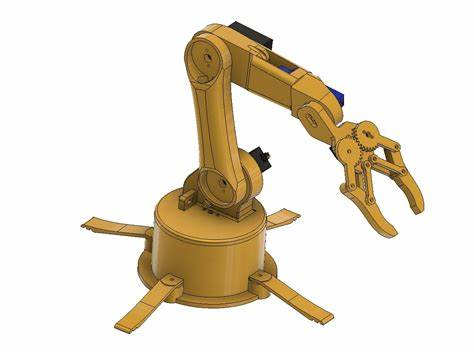
\includegraphics[scale=0.4]{brazo.jpeg}
	\caption{Partes de un brazo robótico articulado de 2 GDL, sin contar el del efector final}
	\label{fig:brazoR}
\end{figure}

\newpage
Sistemas Eléctricos de Potencia Computarizada (SEPDC) es una empresa mexicana que se dedica a fabricar la serie Kaab de Controladores Lógicos Programables (PLC), computadoras especializadas para la automatización industrial (tienen inmunidad al ruido eléctrico y resistencia a la vibración y al impacto). Cada uno de ellos puede ser operado de forma remota a través de un software llamado SettDev. En la Figura \ref{fig:plc} se muestra el PLC-Kaab.

\begin{figure}[htb]
	\centering
	\includegraphics[scale=0.9]{plckaab.png}
	\caption{PLC-Kaab fabricado por SEDPC}
	\label{fig:plc}
\end{figure}

Los PLC´s son empleados para el control de sistemas, como lo demuestra la Figura \ref{fig:siscritico}. Por medio de una versión del software SettDev instalado en el PLC, se monitorea una planta de agua tratada, determinando los niveles de llenado del tanque.

\begin{figure}[htb]
	\centering
	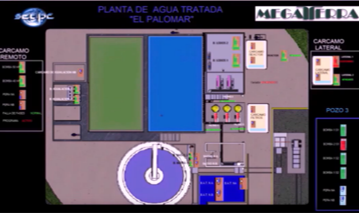
\includegraphics[scale=0.9]{sistemaplc.png}
	\caption{Uso del PLCKaab para controlar un sistema de llenado de agua}
	\label{fig:siscritico}
\end{figure}

\newpage
\section{Planteamiento del problema}

SEDPC necesita un sistema para el control de servomotores que pueda ser instalado sin requerir una configuración exhaustiva para controlar brazos robóticos de diferentes longitudes de 2 DoF, y darle instrucciones al robot por medio del movimiento del brazo de un operador.
\newline\newline\newline
Configurar los grados de libertad de un brazo para llegar a una posición deseada es un problema clásico de la robótica llamado cinemática inversa. Existen métodos algebraicos, geométricos e iterativos para resolverlo, sin embargo, dependen de una configuración de longitud de articulaciones en particular, además de que consumen una gran cantidad de recursos computacionales, lo que dificulta su uso en un dispositivo de bajas prestaciones.

\newpage
\section{Objetivo general}

Desarrollar e implementar un sistema de control utilizando una Raspberry Pi, sensores inerciales y una red neuro-difusa, para controlar la posición del efector final de un brazo robótico de 2 DoF de longitud variable.

\newpage
\section{Objetivos específicos}
\begin{itemize}
	
	\item Desarrollar e implementar un programa en C++, utilizando los ángulos de inclinación en los tres ejes obtenidos por los sensores MPU6050, para determinar la posición del sensor en el extremo de la ortesis de brazo.
	
	\item Implementar la comunicación entre la Raspberry Pi y el software SettDev por medio de sockets TCP en C++ y C\# para enviar los ángulos de inclinación calculados al software, para poder guardar los datos y permitir reproducirlos en la simulación en 3D de un brazo robótico.
	
	\item Desarrollar e implementar una interfaz gráfica de usuario utilizando una pantalla táctil por medio del framework Qt para visualizar la cinemática inversa del brazo robótico a controlar.
	
	\item Desarrollar e implementar en SettDev la comunicación entre el módulo del brazo robótico en 3D y el PLC por medio de sockets UDP en C\# para enviar los ángulos de inclinación al controlador y reproducir los ángulos de inclinación en los servomotores posicionales.
	
	\item Implementar un sistema de inferencia neuro-difuso adaptativo (red neuronal ANFIS) utilizando C++ para resolver el problema de la cinemática inversa del brazo.
	
	\item Desarrollar e implementar un algoritmo de aprendizaje no supervisado utilizando C++ para entrenar la red neuronal.
	
\end{itemize}

\newpage
\section{Justificación}

La determinación de la posición del efector final por medio de sensores inerciales permitirá que el operador pueda dar instrucciones al robot sin que sea necesario que determine manualmente las coordenadas de la posición en el espacio del efector final. Además, la solución a la cinemática inversa no dependerá, dentro de los límites establecidos, de la longitud en particular de cada brazo robótico a ser controlado. Asimismo, será una aplicación práctica de las investigaciones previas a este trabajo sobre el control de un brazo robótico con una red neuro-difusa.

\newpage
\chapter{}

\section{Estado del arte}

\begin{table}[h]
	\caption{Estado del arte}
	\centering
	\begin{tabular}{p{5cm}p{4cm}p{3.6cm}p{5cm}}
		\textbf{Título} & \textbf{Autores} & \textbf{Tipo de publicación, lugar y fecha} & \textbf{Descripción} \\ 
		\midrule
		FIKA: A Conformal Geometric Algebra Approach to a Fast Inverse Kinematics Algorithm for an Anthropomorphic Robotic Arm \newline\newline
		FIKA: Un enfoque de álgebra geométrica conforme para un eficaz algoritmo cinemático inverso para un brazo robótico antropomórfico &  
		Oscar Carbajal-Espinosa; Leobardo Campos-Macías; Miriam Díaz-Rodríguez \newline\newline
		Instituto Tecnológico y de Estudios Superiores de Monterrey; Intel Corporation; Tecnológico Nacional de México & 
		\begin{center}Artículo \par \includegraphics[width=3cm]{mexico.jpg} \par Mexico \par 2024\end{center} & 
		Propone un método geométrico iterativo de 3 fases para resolver el problema de la cinemática inversa.\newline\newline
		Sin embargo, requiere un tiempo de procesamiento de datos inaceptable en un sistema crítico.\\
		\midrule
		Implementation of singularity-free inverse kinematics for humanoid robotic arm using Bayesian optimized deep neural network. \newline\newline
		Implementación de cinemática inversa sin singularidad para brazo robótico humanoide utilizando una red neuronal profunda optimizada por métodos Bayesianos. &  
		Omur Aydogmus; Gullu Boztas \newline\newline 
		Firat University & 
		\begin{center}Artículo \par \includegraphics[width=3cm]{turquia.png} \par Turquía \par 2024\end{center} & 
		Utiliza una red neuronal basada en aprendizaje profundo para resolver la cinemática inversa en una simulación.\newline\newline Sin embargo, el proyecto no se llevó a una aplicación práctica. \\
	\end{tabular}
\end{table}

\newpage
\begin{table}[htb]
	\caption{Estado del arte (continuación)}
	\centering
	\begin{tabular}{p{3.8cm}p{3.8cm}p{3.8cm}p{3.8cm}}
		\textbf{Título} & \textbf{Autores} & \textbf{Tipo de publicación, lugar y fecha} & \textbf{Descripción} \\ 
		\midrule
		Inverse kinematics solution and control method of 6-degree-of-freedom manipulator based on deep reinforcement learning. \newline\newline
		Solución de cinemática inversa y método de control de un manipulador de 6 grados de libertad basado en aprendizaje de refuerzo profundo. &  
		Chengyi Zhao; Yimin Wei; Junfeng Xiao; Yong Sun; Dongxing Zhang; Qiuquan Guo; Jun Yang \newline\newline 
		University of Electronic Science and Technology of China & 
		\begin{center}Artículo \par \includegraphics[width=3cm]{china.png} \par China \par 2024\end{center} & 
		Propone un algoritmo de aprendizaje por refuerzo que calcula la distancia entre el efector final y la posición deseada. \newline\newline Sin embargo, se volverá ineficaz cuando se adapte a brazos de diferente longitud. \\
	\end{tabular}
\end{table}

\newpage
\section{Marco teórico}

\subsection*{Raspberry Pi 3 B+}
\begin{itemize}
	\item Funciona con un sistema operativo basado en la arquitectura ARMv8
	\item Procesador Broadcom BCM2837 de 1,4 GHz, 1 GB de RAM
	\item Módulo Wi-Fi de 2,4 y 5 GHz
	\item 40 pines Entrada/Salida de Propósito General (GPIO)
	\item Salidas de 3.3 y 5 V, bus I²C
\end{itemize}

\begin{figure}[htb]
	\centering
	\includegraphics[scale=0.5]{raspberrypi.jpg}
	\caption{Raspberry Pi 3 B+}
\end{figure}

\subsection*{Qt}
\begin{itemize}
	\item Optimizada para interfaces gráficas en sistemas portátiles
	\item Soporte para C++
	\item Utiliza el lenguaje declarativo QML para programar la interfaz
	\item Soporta hilos para dividir las operaciones
\end{itemize}

\begin{figure}[htb]
	\centering
	\includegraphics[scale=0.5]{qt.jpg}
	\caption{Logotipo de Qt Framework}
\end{figure}

\subsection*{Bus I2C}
\begin{itemize}
	\item Bus serial de comunicación de tipo maestro-esclavo.
	\item Línea serial de datos bidireccional (SDA)  y línea serial de reloj (SCL).
	\item Espacio de direcciones, cada dirección identifica a un dispositivo conectado al bus.
\end{itemize}

\begin{figure}[htb]
	\centering
	\includegraphics[scale=0.5]{i2c.png}
	\caption{Diagrama del bus I2C}
\end{figure}

\subsection*{Bus SPI}
\begin{itemize}
	\item Bus serial de comunicación de tipo maestro-esclavo.
	\item Líneas de entrada al esclavo (MOSI) y salida al esclavo (MISO), línea de reloj (SCLK).
	\item Línea de selección del chip (SS).
\end{itemize}

\begin{figure}[htb]
	\centering
	\includegraphics[scale=0.5]{spi.png}
	\caption{Diagrama del bus SPI}
\end{figure}

\subsection*{MPU-6050}
\begin{itemize}
	\item Giroscopio de vibración de Coriolis y acelerómetro de 3 ejes.
	\item Procesador de movimiento digital (DMP) que mide la orientación del sensor en tres ejes.
	\item Buffer FIFO interno.
	\item Filtro paso bajo.
	\item Comunicación por medio del bus I²C de hasta 400 KHz.
	\item Pin AD0 para cambiar la dirección en el bus. Solo puede tomar las direcciones 104 y 105.
\end{itemize}

\begin{figure}[htb]
	\centering
	\includegraphics[scale=0.5]{mpu6050.jpg}
	\caption{Sensor inercial MPU6050}
\end{figure}

\subsection*{MPU-9250}
\begin{itemize}
	\item Giroscopio de vibración de Coriolis y acelerómetro de 3 ejes.
	\item Procesador de movimiento digital (DMP) que mide la orientación del sensor en tres ejes.
	\item Buffer FIFO interno.
	\item Filtro paso bajo.
	\item Comunicación por medio del bus SPI de hasta 10 MHz.
\end{itemize}

\begin{figure}[htb]
	\centering
	\includegraphics[scale=0.4]{mpu9250.jpg}
	\caption{Sensor inercial MPU9250}
\end{figure}

%\subsection*{Sensor flexible capacitivo}
%\begin{itemize}
%	\item Mide el ángulo de torsión al que se somete el sensor en una dirección.
%	\item El valor medido es una resistencia variable
%\end{itemize}

%\begin{figure}[htb]
%	\centering
%	\includegraphics[scale=0.6]{flexsensor.jpg}
%	\caption{Sensor flexible capacitivo}
%\end{figure}

%\subsection*{Convertidor analógico-digital MCP3004}
%\begin{itemize}
%	\item Voltaje de referencia de 2,7 V a 5,5 V
%\end{itemize}

%\begin{figure}[htb]
%	\centering
%	\includegraphics[scale=0.6]{mcp3004.jpg}
%	\caption{Convertidor A/D MCP3004}
%\end{figure}

\subsection*{Microservomotor posicional}
\begin{itemize}
	\item Ángulo de entrada de 0° a 180°
	\item Utiliza señales de modulación de ancho de pulso (PWM)
	\item Movimiento bidireccional
\end{itemize}

\begin{figure}[htb]
	\centering
	\includegraphics[scale=0.6]{servomotor.png}
	\caption{Microservomotor posicional}
\end{figure}

\newpage
\section{Propuesta de solución}

La empresa requirió que las soluciones de la cinemática inversa se guardaran en un archivo, que posteriormente sea reproducido y enviado desde el software SettDev al PLC-Kaab. De este modo, la propuesta de solución se dividió en dos fases. La Figura \ref{fig:fasecaptura} muestra la primera fase, la de captura de datos. En la etapa de Sensado, el sensor MPU-6050 mide la orientación del sensor, y envía los ángulos de inclinación $S(\theta_x, \theta_y, \theta_z)$ calculados en los 3 ejes a la Raspberry Pi. Estos valores son la entrada de la etapa de Localización, en la cual se determina la posición $(x, y, z)$ en el espacio de la muñeca respecto al hombro (quien tiene la posición $(0, 0, 0)$), que será la que deberá alcanzar el efector final. Estas coordenadas sirven como entrada a la red neuro-difusa en la etapa de Procesamiento, donde, de acuerdo con la longitud de las articulaciones $(L_1, L_2)$ especificada, se calculan los ángulos $(\alpha_1, \alpha_2, \alpha_3)$ que resuelven la cinemática inversa para alcanzar la posición $(x, y, z)$ previamente calculada. Estos ángulos se aplican al movimiento de un modelo de brazo robótico en 2D en una interfaz gráfica en la etapa de Visualización, en la que se puede simular el comportamiento que tendría el brazo robótico al aplicar dichos ángulos, así como al movimiento de un modelo de brazo robótico en 3D en la etapa de Referencia. Finalmente, los ángulos $(\alpha_1, \alpha_2, \alpha_3)$ son almacenados en un archivo con extensión .bin.

\begin{figure}[htb]
	\centering
	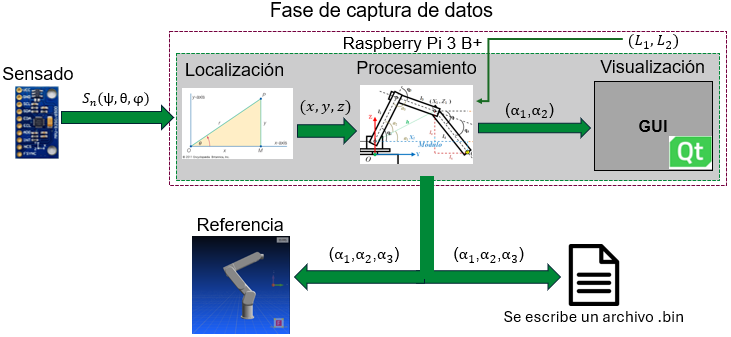
\includegraphics[scale=0.85]{fasecaptura.png}
	\caption{Fase de captura de datos}
	\label{fig:fasecaptura}
\end{figure}

\newpage
La Figura \ref{fig:faseejecucion} muestra la segunda fase, la de ejecución. El archivo con extensión .bin previamente guardado es leído y transmitido por el software SettDev hacia el PLC-Kaab, quien interpreta los ángulos recibidos y los modula en ancho de pulso para controlar la posición de los servomotores posicionales.

\begin{figure}[htb]
	\centering
	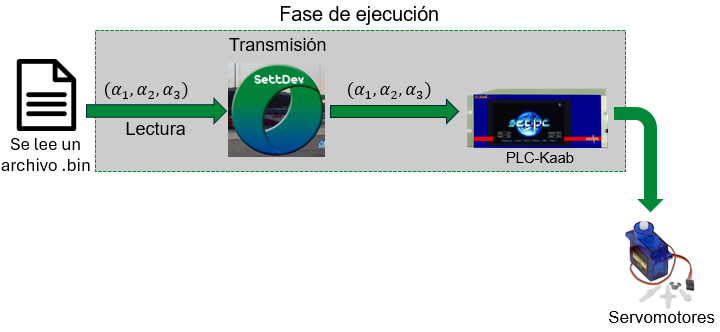
\includegraphics[scale=0.85]{faseejecucion.png}
	\caption{Fase de ejecución}
	\label{fig:faseejecucion}
\end{figure}

\newpage
\chapter{}

\section{Fase de captura de datos}

\subsection{Sensado}

La empresa requirió que se utilizara una ortesis de brazo donde se montara el sistema de medición de los sensores inerciales y la Raspberry Pi. La Figura \ref{fig:ortesis} muestra la ortesis de brazo utilizada. Para encontrar la posición del efector final, se utilizaron dos sensores MPU-6050; uno se colocó en el codo, mientras que el segundo se colocó en el extremo de la ortesis.

\begin{figure}[htb]
	\centering
	{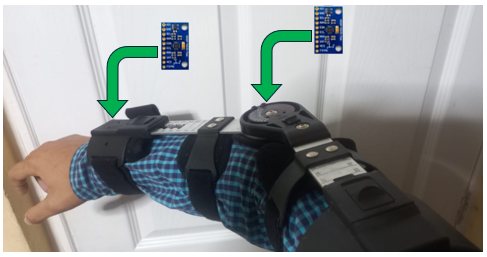
\includegraphics[scale=0.8]{ortesis.png}}
	\caption{Ortesis utilizada para el proyecto}
	\label{fig:ortesis}
\end{figure}

Se realizó la conexión entre los sensores y la Raspberry Pi 3 B+. La Figura \ref{fig:diagrama} muestra el diagrama de interconexión. Los pines SDA y SCL de los sensores MPU-6050 se conectaron al bus serial $I^2C$, mientras que los pines MISO, MOSI y SCK del sensor MPU-9250 se conectaron al bus serial SPI.

\begin{figure}[htb]
	\centering
	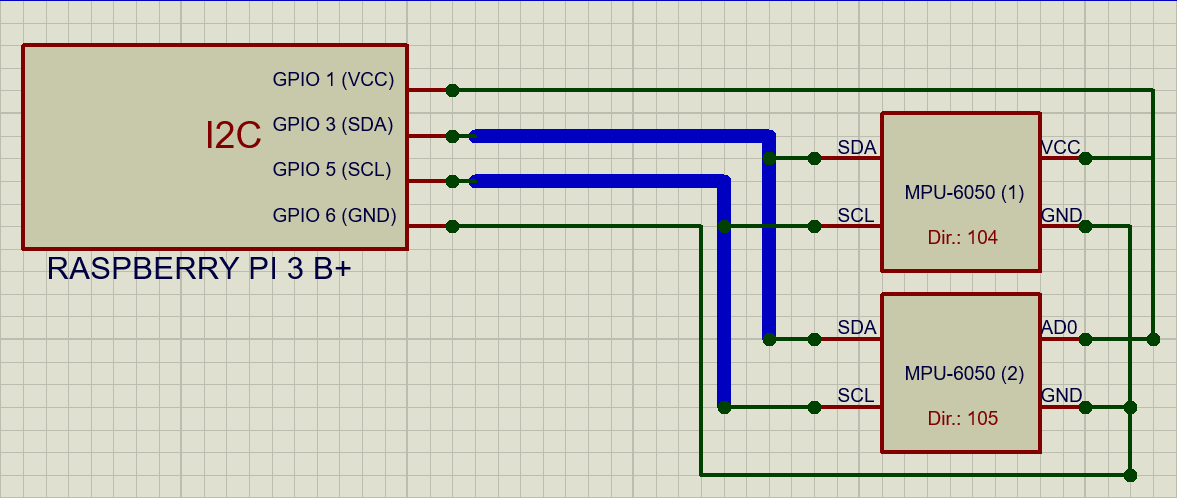
\includegraphics[scale=0.4]{diagrama.png}
	\caption{Diagrama de interconexión entre la Raspberry Pi y los sensores}
	\label{fig:diagrama}
\end{figure}

La línea SS del sensor MPU-9250 se conectó a la línea Chip Enable (CE) 1 de la Raspberry Pi. Nótese que tanto las líneas de datos (SDA), como las líneas de reloj (SCL) de los sensores MPU-6050, se conectaron a una única línea SDA o SCL, respectivamente, hacia la Raspberry Pi. Para evitar problemas de sincronización, se eligió la misma frecuencia de reloj para ambos sensores. Nótese también que se alimentó al sensor a través de la entrada AD0, en vez de VCC. Esto permite que su dirección en el bus $I^2C$ cambie de 104 a 105. Todos los sensores se alimentaron a través de la salida de voltaje de 3,3 V de la Raspberry Pi.

En lo que resta del documento, cuando se haga referencia a los sensores MPU-6050 y MPU-9250 en conjunto, se utilizará el prefijo MPU; cuando se haga referencia solo a uno de ellos, se hará con su nombre completo.

\subsubsection{Calibración}

Los sensores inerciales fabricados con tecnología MEMS, como los MPU, necesitan ser calibrados y tener un valor de referencia (offset) con el cual se corrija la orientación medida por el sensor \cite{offsetMPU}. El diagrama de la Figura \ref{fig:salidaMPU} obtenido del manual \cite{offsetMPU} muestra el proceso para obtener datos de los sensores MPU; los valores de referencia del acelerómetro y el giroscopio (Gyro and Accel Offset Registers) se aplican a las mediciones obtenidas por el giroscopio y el acelerómetro (Gyro and Accel MEMS), para corregir la mediciones y colocarlas en los registros del sensor (Gyro/Accel Output Registers). Luego, son procesadas por el Procesador de Movimiento Digital (DMP) y el resultado se almacena en un buffer FIFO interno.

\begin{figure}[htb]
	\centering
	\includegraphics[scale=0.8]{salidaMPU.png}
	\caption{Lectura de datos de los sensores MPU}
	\label{fig:salidaMPU}
\end{figure}

%El buffer FIFO de los MPU permite implementar un patrón de arquitectura de segmentación de procesos (process pipeline); los datos obtenidos del DMP se colocan en un buffer interno del sensor de tipo FIFO (El primer dato que entra, es el último que sale), del cual se lee la orientación del sensor; esto permite que los datos de la orientación puedan ser procesados sin que existan errores debido a lecturas incompletas. Aunque no se indica explícitamente la estructura de datos interna del buffer, se puede representar como un buffer compartido, esto es, una cola circular. La Figura \ref{fig:buffer} muestra el buffer compartido. Puede notarse que se modela de tal manera que el proceso productor (el DMP) y el proceso consumidor (la lectura de datos del sensor) no accedan al mismo valor.

%\begin{figure}[htb]
%	\centering
%	\includegraphics[scale=0.9]{buffer.png}
%	\caption{Representación del buffer interno del MPU como un buffer compartido}
%	\label{fig:buffer}
%\end{figure}

\newpage
La Figura \ref{fig:ejes} muestra los ejes de desplazamiento y la rotación de los sensores MPU. Se colocaron los sensores MPU en la ortesis de modo que el sentido positivo del eje X quedara hacia el frente del operador (quien tiene colocada la ortesis); de acuerdo con esto, el sentido positivo de rotación en el eje Z se obtiene girando el brazo hacia la izquierda del operador; el sentido positivo de rotación en el eje Y se obtiene girando el brazo hacia abajo; y el sentido positivo de rotación en el eje X se obtiene rotando el brazo hacia la derecha.

\begin{figure}[htb]
	\centering
	\includegraphics[scale=0.5]{ejes.jpeg}
	\caption{Orientación de los ejes y polaridad de rotación de los sensores MPU}
	\label{fig:ejes}
\end{figure}

Se eligieron los valores de referencia de modo que la salida del sensor en el inicio del proceso de medir la orientación fuera $X=0, Y=0, Z=0$ para el giroscopio y $X=0, Y=0, Z=-9.8$ para el acelerómetro, debido a la constante de la aceleración de la gravedad g = -9.8  $m/s^2$. De acuerdo con lo anterior, al procesar los datos por el DMP, la salida deseada en el inicio del proceso de medir la orientación sería $\theta_x = 0°,\theta_y = 0°,\theta_z = 0°$.

Si el sensor se encuentra en estado de reposo (no existe ninguna fuerza externa que lo mueva), se espera que al leer datos de él, los valores no cambien; en la práctica, estos valores pueden variar debido a interferencias como el ruido externo. De modo que se calcula un valor medio cuyo error (la diferencia entre la medición del sensor en estado de reposo y el valor medio) sea menor que un error máximo aceptable; con base en la experiencia, se eligió un error máximo de 0.1 $\degree/s$ para el giroscopio, y 0.1 $m/s$ para el acelerómetro.

Para obtener dicho valor medio, se utilizó un control proporcional-integral (PI), en el cual se escribe el valor medido por el sensor en los registros de referencia (offset registers), y se compara dicho valor con la siguiente medición del sensor (con el último offset escrito en los registros de referencia aplicado a la nueva medición), para determinar el error; este proceso termina cuando el error obtenido se encuentra dentro del rango previamente establecido.

La Figura \ref{fig:calibracion} muestra el proceso de calibración del sensor. A cada medición se le aplicó el control PI para corregir el error. Para permitir que se establezca un valor apropiado, este proceso se repite 600 veces, un valor elegido basado en la experiencia. Después de que termina el ciclo, se compara el siguiente valor del sensor con los valores de referencia en los registros para determinar el error. Si éste es mayor que el error máximo aceptado, se repite el proceso.

Para que la calibración sea adecuada y se obtenga una medición confiable, el sensor debe de encontrarse en el estado de reposo mencionado anteriormente.

\begin{figure}[htb]
	\centering
	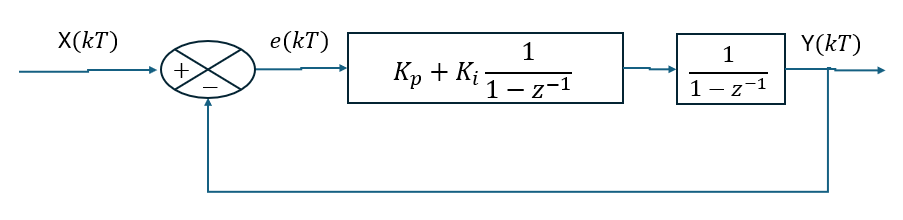
\includegraphics[scale=0.8]{calibracion.png}
	\caption{Diagrama a bloques del proceso de calibración del sensor}
	\label{fig:calibracion}
\end{figure}

\newpage
Posteriormente, se debe de cargar el firmware del procesador \cite{userguideMotionDriver}. Este proceso debe de realizarse cada vez que se encienda el sensor. Aunque no se indique explícitamente, el hecho de que el firmware deba de ser cargado cada vez que se inicie el sensor sugiere que la memoria que contiene el firmware del sensor es una memoria volátil. La memoria está formada por 8 bancos, en los que se carga el firmware proporcionado por InvenSense \cite{userguideMotionDriver}. 

Después de esto, se habilita el DMP y el buffer FIFO escribiendo el valor 1 en el bit FIFO\_EN (Bit 6) del registro 106 indicado en la Figura \ref{fig:fifoen} para la lectura de datos.

\begin{figure}[htb]
	\centering
	\includegraphics[scale=1]{fifoenable.png}
	\caption{Registro User Control del MPU, donde se encuentra el bit (Bit6) para activar el buffer FIFO}
	\label{fig:fifoen}
\end{figure}

\subsubsection{Medición}

El algoritmo utilizado por el DMP para obtener la orientación, no es de dominio público; en el Capítulo \ref{cap:anexos}, se describe el posible algoritmo utilizado por el DMP. Por otro lado, InvenSense, el desarrollador del sensor, ofrece un conjunto de bibliotecas para trabajar con el DMP \cite{userguideMotionDriver}.

%La Figura muestra el proceso general para obtener la orientación del sensor. Primero, se obtiene en el buffer FIFO la orientación obtenida por el DMP, representada internamente por un cuaternión. El cuaternión es rápidamente computable y evita problemas que se producen al girar más de 90°, como el bloqueo del cardán. Posteriormente, se obtiene el vector de gravedad; este permite calcular la aceleración de la gravedad que experimenta el sensor en los 3 ejes, para tomarlo como sesgo y corregir la medición. Por último, se convierte lo antes calculado a valores de Euler, en radianes, y finalmente, dichos valores son convertidos a su equivalente en grados, que son los que se utilizan para indicar la orientación del sensor.

%\begin{figure}[htb]
%	\centering
%	\includegraphics[scale=1]{fifoenable.png}
%	\caption{Determinación de la orientación del sensor}
%	\label{fig:orientacion}
%\end{figure}

El DMP representa internamente la orientación por medio de cuaterniones unitarios. Son rápidamente computables, y evitan problemas que se producen al girar más de 90\degree, como el bloqueo del cardán.

El cuaternión es de la forma:.

\begin{equation}
	q = a + b\hat{i} + c\hat{j} + d\hat{k}
	\label{eq:eqcuaternion}
\end{equation}

Donde $a, b, c, d$ son las componentes del cuaternión que describe la rotación actual del sensor.

Para poder obtener la rotación del sensor, se utilizó la formula que obtiene las nuevas componentes de un vector si se le aplica una rotación descrita por un cuaternión, la cual es la siguiente:

\begin{equation}
	v' = q\cdot v\cdot q*
	\label{eq:rotacioncuaternion}
\end{equation}

Donde $v'$ es el nuevo vector con la rotación aplicada, y $q*$ es el cuaternión conjugado, de la forma:

\begin{equation}
	q* = a - b\hat{i} - c\hat{j} - d\hat{k}
	\label{eq:eqcuaternionconj}
\end{equation}

De acuerdo con los valores de referencia definidos para el acelerómetro ($X=0, Y=0, Z=-9.8$), el vector de gravedad es $g = (0, 0, -1)$.

Se sustituyó en la ecuación \ref{eq:rotacioncuaternion} $v$ por el vector de gravedad. Al resolver para $v'$, se obtuvieron las siguientes ecuaciones para obtener cada componente:

\begin{equation}
	v'_x = 2\cdot(x \cdot z - w \cdot y)
	\label{eq:componentex}
\end{equation}

\begin{equation}
	v'_y = 2\cdot(w \cdot x + y \cdot z)
	\label{eq:componentey}
\end{equation}

\begin{equation}
	v'_z = w^2 - x^2 - y^2 + z^2
	\label{eq:componentez}
\end{equation}

Para obtener los ángulos entre el vector $v'$ y los ejes $x$, $y$, $z$ definidos cuando se calibró el sensor (es decir, aquella orientación del sensor en la que la salida del DMP es $\theta_x = 0°,\theta_y = 0°,\theta_z = 0°$), se utilizaron las siguientes ecuaciones:

\begin{equation}
	\theta_x = \tan^{-1}\frac{v'_y}{v'_z}
	\label{eq:angulox}
\end{equation}

\begin{equation}
	\theta_y = \tan^{-1}\frac{v'_x}{\sqrt{v'^2_y + v'^2_z}}
	\label{eq:anguloy}
\end{equation}

\begin{equation}
	\theta_z = \tan^{-1}\frac{q_x \cdot q_y + q_w \cdot q_z}{1 - 2 \cdot (q_x^2 + q_y^2)}
	\label{eq:anguloz}
\end{equation}

Si el sensor se encuentra boca abajo (es decir, la componente Z del vector de gravedad apunta en el sentido positivo del eje Z), es necesario invertir el sentido de la inclinación en el eje Y. Si el valor de la inclinación en el eje Y es positivo, el valor se corrige a $\pi - v'_y$; si es negativo, el valor se ajusta a $-\pi - v'_y$.

Los ángulos obtenidos $\theta_x$, $\theta_y$, $\theta_z$, son la orientación del sensor.

\subsection{Localización}

La posición $P(x, y, z)$, en centímetros, del sensor en el extremo de la ortesis, será la posición que debe alcanzar el efector final del brazo robótico. Esta se mide con respecto al hombro, que tiene las coordenadas en el origen $(0, 0 ,0)$.

Si $(\psi_{1}, \theta_{1}, \phi_{1})$ son los ángulos de inclinación obtenidos del sensor colocado en el codo de la ortesis, y $(\psi_{2}, \theta_{2}, \phi_{2})$ son los ángulos de inclinación obtenidos del sensor colocado en el extremo de la ortesis, las siguientes ecuaciones permiten calcular las coordenadas en el espacio del sensor en el extremo de la ortesis con respecto al hombro \cite{tailtbryan}:

\begin{equation}
x = L_1 \cos(\psi_1) \cos(\theta_1) + L_2 \cos(\psi_2) \cos(\theta_2)
\end{equation}

\begin{equation}
y = L_1 \sen(\psi_1) \cos(\theta_1) + L_2 \sen(\psi_2) \cos(\theta_2)
\end{equation}

\begin{equation}
z = L_1 \sen(\theta_1) + L_2 \sen(\theta_2)
\end{equation}

Donde $L_1$ es la distancia desde el hombro hasta el sensor colocado en el codo, y $L_2$ es la distancia desde el sensor colocado en el codo hasta el sensor colocado en el extremo de la ortesis. La ortesis mide 21 cm en cada articulación, de modo que $L_1 = L_2 = 42$.

El resultado es el que se muestra en la Figura \ref{fig:resultante}. Las componentes antes calculadas permiten obtener la resultante, cuya punta es la posición $P(x,y,z)$ calculada del efector final. Este procedimiento se llama cinemática directa; a partir de los ángulos que describen la postura del robot, se determina la posición que alcanza en el espacio.

\begin{figure}[htb]
	\centering
	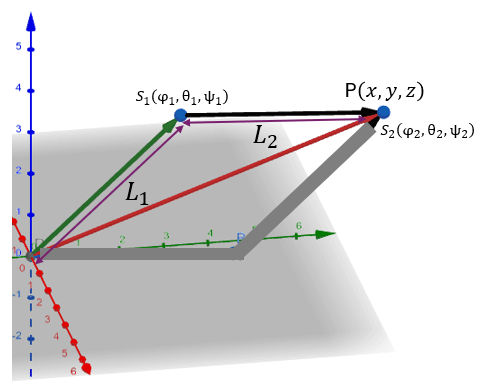
\includegraphics[scale=0.5]{resultante.png}
	\caption{Cálculo de la resultante para obtener la posición del efector final}
	\label{fig:resultante}
\end{figure}

\subsection{Procesamiento}

Para generar el conjunto de datos de entrenamiento para la red se tomaron en cuenta restricciones sobre el brazo robótico a controlar y los servomotores posicionales a los que se envían las instrucciones.

El tipo de brazo robótico a controlar tiene un diseño antropomórfico, lo que significa que se compone de articulaciones unidas entre sí; además es de dos grados de libertad, lo que implica que tiene exactamente dos articulaciones. Como lo que interesa es controlar la posición (y no la orientación), se restringió la cantidad de grados de libertad del brazo robótico a uno en cada unión; esto significa que en la unión de la base existe un grado de libertad, y el otro grado de libertad se encuentra en la unión entre la primera y la segunda articulación. Además, ambos grados de libertad se mueven de arriba hacia abajo. Para alcanzar todas las posiciones, . La Figura \ref{fig:tipobrazo} muestra un ejemplo de un brazo robótico que cumple con estas restricciones.

\begin{figure}[htb]
	\centering
	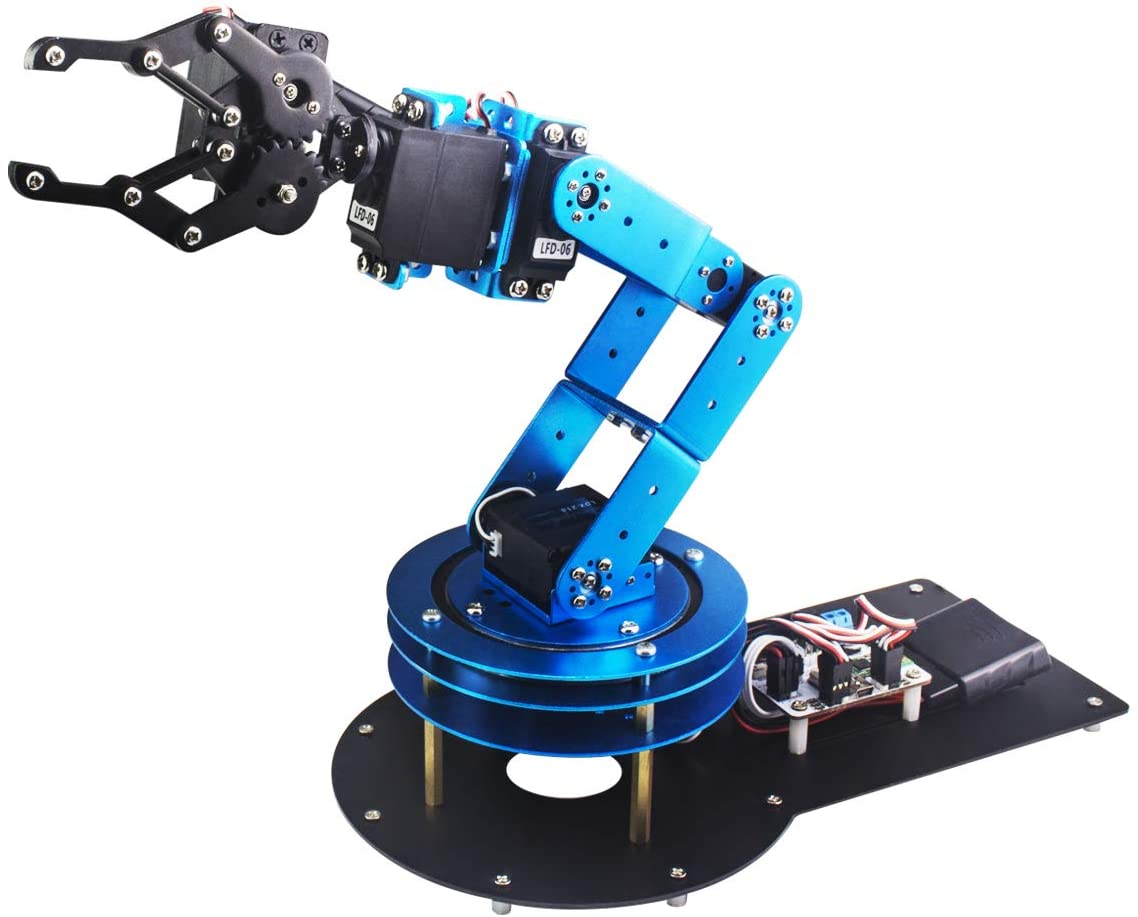
\includegraphics[scale=0.5]{tipobrazo.png}
	\caption{Brazo robótico de 2 DoF que cumple las restricciones impuestas}
	\label{fig:tipobrazo}
\end{figure}

Los servomotores posicionales solo pueden moverse en ángulos discretos, en particular, enteros. Esto significa que pueden alcanzar 180 posiciones. Además, muchas posiciones finales son lo suficientemente cercanas entre sí como para considerar que se aproximan a la misma posición.  Para determinar la proximidad de las posiciones, se aplicó el siguiente criterio con distancia Euclidiana entre dos posiciones $P_1 = (x_1, y_1, z_1)$ y $P_2 = (x_2, y_2, z_2)$:

\begin{equation}
	d(P_1, P_2) = \sqrt{(x_2 - x_1)^2 + (y_2 - y_1)^2 + (z_2 - z_1)^2} < 1
\end{equation}

De este modo, se considera que aquellos puntos a menos de 1 cm de distancia euclidiana entre ellos llegan a la misma posición. 

El brazo robótico tiene la base en el suelo; esto significa que se puede mover dentro y a lo largo de la mitad de una esfera con centro en la base del robot y de radio igual a la longitud del robot.

\subsection{Visualización}

La empresa requirió que se mostrara en una interfaz gráfica un brazo en 2D controlado con los ángulos calculados de la cinemática inversa.

Para desarrollar la aplicación, se utilizó el framework Qt, en el cual se implementaron las etapas de Sensado y Localización en C++. La interfaz se implementó en QML, un lenguaje declarativo que facilitó el desarrollo de la interfaz.

El proceso de lectura de datos del sensor se ejecuta constantemente, lo que puede bloquear los procesos de la interfaz y que ésta deje de responder para el usuario. Para evitar dicho problema, se colocó dicho proceso de lectura de datos en un hilo; éste permite que un subproceso pueda ejecutarse de forma concurrente con otros subprocesos. Para que el hilo de captura de datos pueda comunicar las lecturas a la interfaz, y que éstas puedan ser visualizadas en la interfaz gráfica, se utiliza el paso de mensajes; Qt permite enviar mensajes entre hilos a través de señales. De este modo, también se evitan problemas de concurrencia si ambos hilos intentan acceder a la misma variable donde se almacenan los datos de los sensores.

En la Figura \ref{fig:interfaz} se observa el brazo en 2D; puede notarse que se indica el plano que está siendo visualizado; esto puede ser configurado con el botón arriba a la izquierda. También puede observarse la posición del efector final determinada por la etapa de localización. La gráfica está graduada, de modo que se puede apreciar la precisión del modelo.

\begin{figure}[htb]
	\centering
	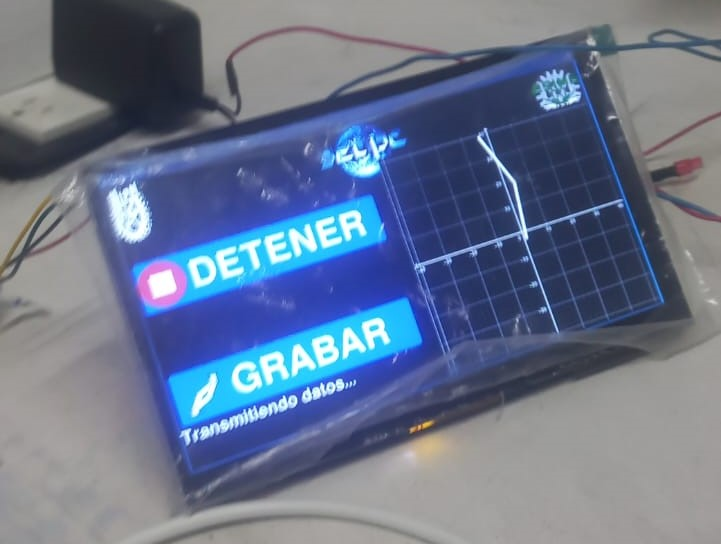
\includegraphics[scale=0.5]{interfaz.jpg}
	\caption{Interfaz gráfica de usuario mostrada en la pantalla táctil de la Raspberry Pi}
	\label{fig:interfaz}
\end{figure}

\subsection{Referencia}

\subsubsection{Transmisión}

Se implementó en C++ y C\# la funcionalidad para transmitir los datos entre la Raspberry Pi y el software SettDev. Dicho software se ejecuta en el sistema operativo Windows; para este trabajo, se ejecutó en la versión Windows 10.

\subsubsection{Simulación}

En la Figura \ref{fig:settdev} se observa la interfaz de usuario de SettDev. Éste se compone por módulos; cada módulo es un componente que interactúa con una característica en particular del PLC que se controla desde el software. La interfaz que se muestra, es el módulo desarrollado por personal de SEDPC para el proyecto; éste contiene un modelo en 3D de un brazo robótico, en el que las inclinaciones de cada una de sus articulaciones son modificadas por los controles deslizantes que aparecen en la parte superior del modelo.

\begin{figure}[htb]
	\centering
	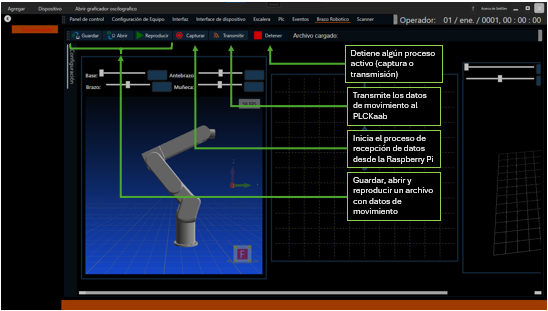
\includegraphics[scale=0.9]{settdev.png}
	\caption{Módulo de Brazo Robótico desarrollado por SEDPC}
	\label{fig:settdev}
\end{figure}

La Figura \ref{fig:referencia} muestra en detalle el brazo en 3D, modelado por personal de SEDPC. Este modelo tiene 2 grados de libertad (además del de la base), y un grado de libertad adicional para el efector final (Muñeca). Este brazo robótico recibirá los ángulos de inclinación de la etapa de Procesamiento y los reproducirá.

\begin{figure}[htb]
	\centering
	\includegraphics[scale=0.6]{referencia.png}
	\caption{Modelo de brazo en 3D utilizado como referencia}
	\label{fig:referencia}
\end{figure}

\newpage
\newpage
\subsection{Almacenamiento}

Los ángulos recibidos en el software SettDev se almacenaron en un archivo binario. Este archivo contiene las instrucciones en conjuntos de 4 bytes, de acuerdo con lo mencionado en la trama utilizada para la transmisión.

\newpage
\section{Fase de ejecución}

\subsection{Lectura}

Se implementó la funcionalidad en el software SettDev para leer y reproducir un archivo. La Figura \ref{fig:cargaarchivo} muestra el proceso de carga de un archivo. El programa permite abrir un cuadro de diálogo para seleccionar un archivo del equipo, de tipo .bin. Cuando se da clic al botón ``Abrir'' y se cierra el archivo, el programa verifica la extensión del archivo. Posteriormente, comienza a leer los datos del archivo.

\begin{figure}[htb]
	\centering
	\includegraphics[scale=0.65]{cargaarchivo.png}
	\caption{Módulo de carga de archivo implementado en SettDev}
	\label{fig:cargaarchivo}
\end{figure}

\subsection{Transmisión}

Se desarrolló e implementó la comunicación entre el software SettDev y el PLC para transmitir los datos leídos desde el archivo. El PLC-Kaab de SEDPC se controla y comunica utilizando datagramas; éstos se envían por medio del protocolo UDP, y tienen un formato de trama específico, que es el que se muestra en la Figura \ref{fig:tramaPLC} obtenida de SEDPC. La trama comienza con un encabezado (Header) que siempre contiene el valor 8A, seguido de algunas indicaciones para el PLC, como el proceso Fuente del que provienen los datos, el proceso de Destino, e indicaciones internas (Internal Indications). Luego, se indica un comando (Command), un subcomando (Subcommand), la indicación de algún Error producido, y la longitud $n$ de los datos por enviar (Largo). Los siguientes $n$ bytes contienen la información a enviar (Data). Por último, se calcula un Checksum como medio de comprobación de errores; si se produce algún error, el PLC no reproduce el datagrama enviado. Se utilizan identificadores con valores numéricos para indicar la Fuente o Destino (el proceso) que envía o recibe los datos, así como el comando y subcomando por ejecutar.

\begin{figure}[htb]
	\centering
	\includegraphics[scale=0.4]{tramaPLC.jpg}
	\caption{Formato de trama utilizado por el PLC-Kaab}
	\label{fig:tramaPLC}
\end{figure}

Para enviar los datos al PLC-Kaab, se tomó como referencia  un módulo desarrollado por SEDPC que tiene una interfaz humano-máquina en SettDev para enviar ángulos concretos a servomotores conectados al PLC. En dicha interfaz, existen controles deslizantes que indican los ángulos enviados al PLC; los valores son transmitidos al dar clic a un botón ``Enviar''. La trama generada para enviar los ángulos de inclinación al PLC se diseñó considerando la trama de este módulo, en el que el campo de Datos contiene 1 byte para representar el número de motor a controlar, y 4 bytes en formato Little Endian que representan el ángulo enviado a dicho motor.

En el formato Big Endian, que es el que comúnmente se utiliza para representar un valor digital, los bytes de izquierda a derecha se ordenan desde el más significativo hasta el menos significativo. En el formato Little Endian, este orden se invierte.

\newpage
\chapter{}

\subsection{Pruebas}

Para determinar cómo cambia la precisión del sistema en la generación de los grupos, se variaron los parámetros $L_1, L_2, \alpha_1, \alpha_2, \alpha_3$. En particular, se variaron $L_1$ y $L_2$ de 0.1 cm a 1 cm, y los saltos de $alpha_1, alpha_2, alpha_3$ variaron en saltos de 1 en 1 hasta 5 en 5, sin tomar en cuenta la variación de saltos de acuerdo con el rango de la longitud que se consideró en la etapa de Procesamiento.

\section{Resultados}

El resultado de la métrica de la desviación de la posición final, tomando el máximo valor con $L = 21 cm$, es de 0,65 cm. Dado que no hay un estándar sobre un umbral de precisión para una determinada aplicación, esto último depende de las especificaciones establecidas en el momento de integrarlo en algún sistema.

La comparación de esta precisión con el estado del arte se muestra en la Tabla \ref{Precision}. Cabe resaltar que los trabajos del estado del arte se aplicaron con ángulos no enteros que no son alcanzables por servomotores posicionales, de modo que, para la aplicación específica del robot, su precisión puede verse sesgada.

\begin{table}[ht]
	\centering
	\begin{tabular}{p{5cm}p{4cm}p{3.6cm}p{4cm}}
		\hline
		\textbf{Sistema implementado (cm)} & \textbf{Método iterativo (cm)} & \textbf{Método por clusterización K-Means (cm)} & \textbf{Método geométrico (cm)} \\
		\hline
		0,65 cm & 0,36 cm & 0,45 cm & 0,12 cm \\
		\hline
	\end{tabular}
	\caption{Resultados de la prueba de precisión}
	\label{tab:Precision}
\end{table}

Los resultados de la prueba de eficiencia se muestran a continuación.

\begin{table}[ht]
	\centering
	\begin{tabular}{p{4cm}p{5cm}p{4cm}p{3.6cm}p{4cm}}
		\hline
	    \texbf{ISO} & \textbf{Sistema implementado (cm)} & \textbf{Método iterativo (cm)} & \textbf{Método por clusterización K-Means (cm)} \textbf{Método geométrico} \\
		\hline
		\textbf{Tiempo promedio de generación de los datos / entrenamiento (s)} & 0,65 & 45 & 30 \\
		\textbf{Tiempo promedio del cálculo de la cinemática inversa (ms)} & 0,65 cm & 0,36 cm & 0,45 cm \\
		\textbf{Memoria utilizada durante la ejecución (MB)} & 0,65 cm & 0,36 cm & 0,45 cm \\
		\textbf{Tamaño de los datos almacenados (MB)} & 0,65 cm & 0,36 cm & 0,45 cm \\
		\hline
	\end{tabular}
	\caption{Resultados de la prueba de eficiencia}
	\label{tab:Precision}
\end{table}


\section{Conclusiones}

Finalmente, se concluye que el modelo de clusterización obtenido, pese a requerir una cantidad considerable de tiempo para la generación de datos, posee un tiempo de respuesta muy reducido, lo que no compromete los recursos disponibles de la Raspberry Pi. Además, el tamaño de los archivos de clusterización generados no crece exponencialmente conforme varían las longitudes de las articulaciones, y, conforme aumenten los grados de libertad, el tamaño total aumenta de forma lineal. Incluir más grados de libertad para determinar la posición en el modelo aumenta exponencialmente el tiempo para la generación de datos, lo que requiere una estrategia de optimización si se quiere llevar a dicha aplicación. La precisión del modelo se establece con una cota máxima desde el principio; conforme se disminuya esta cota, se aumentará la aproximación, lo que implica que el tamaño de los clústeres aumentará; no obstante cada clúster mantendrá su tamaño original.

\subsection{Trabajo a futuro}

Como trabajo a futuro, se tiene lo siguiente:

\begin{itemize}
	\item Incorporar el sistema dentro del PLC-Kaab
	\item Ampliar el sistema para brazos robóticos de 3 DoF
	\item Ampliar el sistema para controlar brazos robóticos de longitudes mayores a la de la ortesis
\end{itemize}

\newpage
\renewcommand{\bibname}{Referencias}
\bibliographystyle{IEEEtran}
\bibliography{referencias}

\end{document}